\begin{slikaDesno}{fig/vrste_rl_0.pdf}
\PID \label{z:RL_kolo}
У колу са слике познато је 
$L = 1\unit{mH}$ и $R = 50\unit{\Upomega}$.
У почетном тренутку струја калема је 
$i_{L}(0^-) = 0,5\unit{mA}$. Напон побудног
генератора је облика 
$v_{\rm g}(t) = V_{\rm m} \sin(\upomega t)
\,{\rm u}(t)$, где су
$V_{\rm m} = 1\unit{V}$ и 
$\upomega = 10^6
\unit{\dfrac{rad}{s}}$. 
Као одзив се посматра 
струја калема на отпорнику $i_L = i_L(t)$.
%
Одредити (а) одзив на 
почетне услове, (б) одзив на побуду, 
(в) комплетан одзив и  
(г) устаљени одзив. 
\end{slikaDesno}

\textsc{\underline{Решење}}:
Диференцијална једначина која описује систем је 
\begin{equation}
    L \dfrac{{\de }i_L}{{\de t}} + R i_L = v_{\rm g}.
    \label{difeq}
\end{equation}
Њој одговара карактеристични полином $P(\uplambda) = R + L\uplambda$ који има само један реалан корен 
$\uplambda_0 = -\dfrac{R}{L} = - 5\times 10^4\,{\rm s}^{-1}$. Хомогени део решења ове диференцијалне 
једначине је стога $i_{L,\rm h}(t) = I_0 {\rm e}^{\uplambda_0 t}$, где је $I_0$ произвољна константа.
Партикуларни део се може одредити помоћу поступка показаног за нерезонантну синусоидалну побуду у задатку
\ref{z:sin_cos_pobuda}, према 
\begin{equation}
i_{L, \rm p} = \mathbb I{\rm m}\left\{\dfrac{V_{\rm m}{\rm e}^{{\rm j}\upomega t}}{P({\rm j}\upomega)}
\right\} = 
\mathbb I{\rm m}\left\{
\dfrac{V_{\rm m}{\rm e}^{{\rm j}\upomega t}}{R + {\rm j}\upomega L}
\right\} = V_{\rm m}
\dfrac{ 
R \sin (\upomega t) - 
\upomega L \cos(\upomega t)
}{R^2 + (\upomega L)^2}. 
\end{equation}
Коначно, опште решење за струју калема је
\begin{equation}
i_{L}(t) = 
\underbrace{
I_0 {\rm e}^{\uplambda_0 t} }
_{\text{Хомогени део}}
+ 
\underbrace{
V_{\rm m}
\dfrac{ 
R \sin (\upomega t) - 
\upomega L \cos(\upomega t)
}{R^2 + (\upomega L)^2}}
_{\text{Партикуларни део}}
. 
\end{equation}

\vspace*{1mm}
(а) Одзив на почетне услове налази се само на
основу хомогеног дела, помоћу  
почетних услова. Добија се 
$$i_{L1}(t) = I_{01}{\rm e}^{\uplambda_0 t}
\Rightarrow
 i_{L1}(0^{-}) = 
 I_{01}\cancelto{1}{ {\rm e}^{\uplambda_0 \cdot 0} } \Rightarrow
 I_{01} = 0,5\unit{mA} .
$$
Тако да је одзив на почетне услве 
$i_{L1}(t) = 0,5\unit{mA}\,{\rm e}^{\uplambda_0 t}$. \\


(б) Одзив на побуду, одређује се заменом постиницијалних почетних услова у опште
решење диференцијалне једначине. Приликом тражења одзива на побуду претпоставља се да су сви 
преиницијални услови равни нули. Додатно, уколико у десној страни нема Диракових импулса 
онда су све функције $i_L(t), i_L'(t), i_L''(t), \dots, i_L^{(n-1)}(t)$ 
непрекидне, 
па су стога и постиницијални услови равни нули. У том облику тражи се \textit{другачија} 
константа за хомогени део.
\begin{equation}
\begin{aligned}
\underbrace{i_{L2}(0^+) = 0}
_{\text{Постиницијални услов}} = 
\underbrace{
I_{02} {\rm e}^{\uplambda_0 \cdot 0} }
_{\text{Хомогени део}}
+ 
\underbrace{
V_{\rm m}
\dfrac{ 
R \sin (\upomega \cdot 0) - 
\upomega L \cos(\upomega \cdot 0)
}{R^2 + (\upomega L)^2}
}
_{\text{Партикуларни део}}
& = 
I_{02} + \dfrac{\upomega L V_{\rm m} }{
R^2 + (\upomega L)^2} 
\Rightarrow \\
& = I_{02} \approx 1 \unit{mA}.
\end{aligned}
\end{equation}
Тако да је одзив побуду:
$
i_{L2}(t)
\approx 
1\unit{mA}\, {\rm e}^{\uplambda_0 t} 
+ 
50 \unit{\upmu A}\, \sin(\upomega t) -
1\unit{mA}\,
\cos (\upomega t).
$


\begin{figure}[b!]
    \hspace*{0pt}\hfill
    \begin{subfigure}[t]{0.45\textwidth}
        \centering
        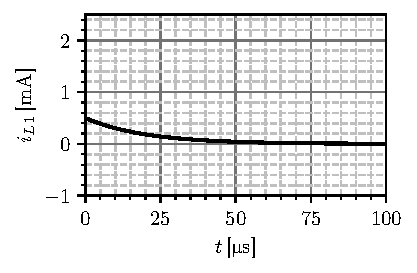
\includegraphics[scale=1]{fig/vrste_rl_1.pdf}
        \caption{Сопствени одзив.}
    \end{subfigure}
    \hspace*{0pt}\hfill
    \begin{subfigure}[t]{0.45\textwidth}
        \centering
        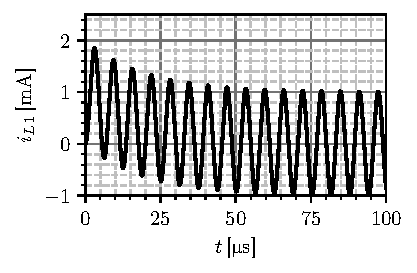
\includegraphics[scale=1]{fig/vrste_rl_2.pdf}
        \caption{Одзив на побуду.}
    \end{subfigure}
    \hfill
    \hspace*{0pt}

    \hspace*{0pt}\hfill
    \begin{subfigure}[t]{0.45\textwidth}
        \centering
        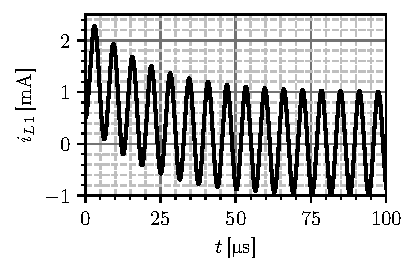
\includegraphics[scale=1]{fig/vrste_rl_3.pdf}
        \caption{Комплетан одзив}
    \end{subfigure}
    \hfill
    \hspace*{0pt}

    \caption{}
    \label{fig:\ID.2}
\end{figure}

(в) На основу суперпозиције, комплетан одзив добија се сабирањем одзива на почетне услове и 
одзива на побуду. Коначан резултат је валидан од тренутка $t=0$ услед чега 
се дописује одскочна функција. Коначно је комплетан одзив:
\begin{equation}
i_L(t) \approx
\bigl(1,5\unit{mA}\,{\rm e}^{\uplambda_0 t}
+
50 \unit{\upmu A}\, \sin(\upomega t) -
1\unit{mA}\,
\cos (\upomega t)
\bigr)
\,\uu(t).
\end{equation}
Приметимо да у овом изразу постоји члан 
добијен из хомогеног дела који је 
побуђен напонским генератором.  \\

(г) Након довољно дугог времена, чланови хомогеног дела који представљају прелазни
режим ишчезавају будући да је 
$e^{\uplambda_0 t} \to 0$ јер је 
$\uplambda_0 < 0$, након чега 
преостаје устаљени одзив
\begin{equation}
i_{L,\rm ss}(t) \approx 
50 \unit{\upmu A}\, \sin(\upomega t) -
1\unit{mA}\,
\cos (\upomega t).
\end{equation}

\vspace*{1mm}
\noindent
Добијени резултати су нацртани на 
дијаграмима на слици \ref{fig:\ID.2}.


